\documentclass[a4paper]{article}

\usepackage[backend=biber, sorting=none]{biblatex}
\usepackage[]{geometry}
\usepackage[font={normalsize,it}]{caption}
\usepackage{titlesec}
\usepackage{graphicx}
\usepackage{subfig}
\usepackage{amsmath}
\usepackage[toc,page]{appendix}
\usepackage{pgfplots}
\usepackage{tikz}

\addbibresource{references.bib}

\renewcommand{\thesection}{\arabic{section}}
\renewcommand{\thesubsection}{\arabic{subsection}}
\renewcommand{\thesubsubsection}{\arabic{subsubsection}}

\titleformat{\section}{\LARGE\sc}{\thesection.}{1em}{}
\titleformat{\subsection}{\normalsize\it}{\thesection.\thesubsection}{0.9em}{}
\titleformat{\subsubsection}{\small\it}{\thesection.\thesubsection.\thesubsubsection}{0.9em}{}


\pgfplotsset{compat=1.11,
	/pgfplots/ybar legend/.style={
		/pgfplots/legend image code/.code={%
			\draw[##1,/tikz/.cd,yshift=-0.25em]
			(0cm,0cm) rectangle (3pt,0.8em);},
	},
}
\begin{document}

\begin{center}

\vspace{1.7cm}

\begin{Huge}
Slum Detection using Multiclass Land Cover in Bangalore
\end{Huge}


\vspace{1.5cm}

Derk Barten\\
11043075

\vspace{1.5cm}

Honors Bachelor thesis extention\\
Credits: 6 EC

\vspace{0.5cm}

Bachelor Opleiding Kunstmatige Intelligentie

\vspace{0.25cm}

University of Amsterdam\\
Faculty of Science\\
Science Park 904\\
1098 XH Amsterdam

\vspace{4cm}

\emph{Supervisor}\\
Dr. Debraj Roy

\vspace{0.25cm}

Department of Computational Science\\
Faculty of Science\\
University of Amsterdam\\
Science Park 904\\
1098 XH  Amsterdam

\vspace{1.5cm}

\today

\end{center}


\clearpage

\section{Introduction}

Informal housing is a common issue faced by cities in developing countries. Inhabitants of informal regions, commonly named as slums, have less social economic opportunities and a lower quality of life compared to urban residents in formal housing. The monitoring of these the development of slums requires resources which governments in developing countries often cannot spare. Remote sensing methods from satellites provide a relatively low cost solution in tracking development of slums in the city. The detection of informal areas from the images provides by satellites remains a difficult task despite the effort from the field of study. This is in part caused by the disparate nature of slums, which varies between cities and even between regions of the same city. The slum characteristics of this type of slum are small buildings which are similar to tents, covered with plastic fabric roofs often colored blue. This type of slum indicates a newly developing slum, which has often a lack of basic services, such as infrastructure and sanitation. Over time, the inhabitants of these slums improve the build quality of the slums into permanent housing. Slum upgrading efforts of the government aim to support these slums by providing the lacking basic services to these newly developed neighborhoods. In this thesis, we focus explicitly on this type of developing slum. The automatic detection of developing slums from satellite images enables the government to support the needs of these developing neighborhoods.

\subsection{Global Context}
% state
According Un-Habitat, close to a third of the global urban population lives in informal settlements \cite{2016state}. In specific parts of the world, for instance Sub-Saharan Africa, the urban population that lives in informal housing is estimated to be close to two thirds of the total urban population \cite{un2013planning}. In the past decades, the percentage of slum inhabitants compared to the urban population has decreased. Paradoxically, in absolute terms, the total number has actually increased \cite{2016state}.

% definition and negative effects
Informal settlements exist globally, although often in different forms and described using different names. The individuals living in informal settlements, such as slum dwellers, are specified by Un-Habitat by one ore more of the following conditions: inadequate  drinking  water,  inadequate  sanitation, poor  structural quality of housing, over crowding and insecurity of tenure \cite{un2015slum}. In addition, the inhabitants of slums experience social and economical exclusion from the opportunities that an urban environment offers. Furthermore, slum dwellers are prone to natural disasters in addition to disease outbreaks. 

% solution
Over the years, there have been multiple governmental policies implemented to address the problem of informal settlements. Informal settlements were largely tolerated and neglected, large eviction and resettlement of the inhabitants were not found to be effective \cite{kuffer2016slums}. Instead, in recent years, a less intrusive approach is used in solving the slum problem. This method enables governments to solve the slum question by supporting the upgrade of slums to formal housing \cite{cobbett2013cities}. Besides government policy, Un-Habitat allocates a significant effort to the use of this method itself\cite{2015globact}.

\subsection{Related works and contributions}
% into remote sensing
In many cities in the developing world, slums are a large part of the urban environment. However, there is often a lack of information about the properties of the slum, such as the location, the scale and the population \cite{kuffer2016slums}. These cities often do not have the resources to obtain this information. Remote sensing is able to provide the often lacking  social economic information. Besides, remote sensing is also able to capture the spatial and temporal dynamics of the informal areas, which supports urban planning and the development of the city.

% methods
In the last decade, access to satellite images was becoming widespread along side an increase in methods for urban area classification \cite{kuffer2016slums}. This allowed for informal areas to be studied throughout the globe, e.g. Colombo \cite{colombo}, Johannesburg \cite{williams2016automatic}, Accra \cite{accra}, Mumbai \cite{mumbai}, Rio de Janeiro \cite{hofmann2008detecting}, and Hyderabad \cite{hyderabad}. With the increase interest in slum detection, it became apparent that the structural characteristics of slums were quite different from formal areas. This led to a large number of approaches based on the extraction of  image based features from satellite images. These approaches are, among others: the presence of vegetation \cite{niebergall2007object}, the size and shapes of buildings \cite{hofmann2008detecting}, the roofing material \cite{williams2016automatic}, texture features \cite{mattia2007exploiting}, and road accesability \cite{owen2013approach}.

Currently, the majority of studies uses the pixel image data of informal regions to extract features \cite{kuffer2016slums}. A different approach would be the characterization of areas by the objects that inhabit them. This is, for example, the detection of individual roofs in a certain area  of an image \cite{williams2016automatic}. Another example of this object based approach is the detection of road systems to characterize image regions. Alternatively, studies have used land use information \cite{novack2010urban} or social economical statistics \cite{engstrom2011using} to detect informal settlements.

% results
% The performance of the methods used in the studies is very variable. There are studies that have achieved a very high accuracy of in the 90\%. 

% conclusion prev work
%Because slums vary incredibly between different cities and regions, it is hard to obtain consensus about characteristics that well define informal areas. This variety makes it hard to create a method that will capture all the types of informal areas. As a result, the results obtained by the studies are quite specific to the studied city or area. 

 
\subsection{Proposed Method}

Our thesis continues with the work performed by Graesser \textit{et al.} \cite{graesser2012image}. The paper characterized formal and informal neighborhoods using a set of different features extracted from satellite images. Their approach was able to successfully characterize the two types of neighborhoods with high accuracy on certain parts of the urban landscape. We will evaluate two of the feature extraction methods described in the paper from Graesser \textit{et al.} and attempt to reproduce similar results with satellite images from Bangalore. These methods are the Histogram of Oriented Gradients and Line support regions. Beyond the replication and evaluation of previous research, the methods of feature extraction used by Graesser \textit{et al.} will be extended with an additional new method. This method creates a feature based on the density of road intersections in an image. The feature created from this method will be compared to the existing features and measured for its performance. The features produced by the three methods will combined and used by a set of different classification methods.
We will evaluate the different classification methods to discover the most suitable classification method for our image and its features. 



\subsection{Data and Area of Study}
The image data used for the thesis is displayed in Figure \ref{fig:sections}d, a larger version of the image is included in appendix A. The content of this image contain a large area of Bangalore, which is the capital city of the Indian state of Karnataka, located in south central India. The city experienced a fast growth population from 8.4 million in 2011 to 12.3 million in 2017, becoming the third largest city in India\cite{popcount2017}. One of the reasons for its sudden growth is the large IT sector together with better living standards and infrastructure. This rapid increase in population has led to a shortage of housing which, in turn, caused an increase in the number slums in the city. At present, the city is estimated to have over two thousand slums. These slums account for 25 to 35 percent of the urban population \cite{roy2018survey}.

The image in Figure \ref{fig:sections}d has a resolution of 52,322 by 31,789 pixels with a filesize of 6.19GiB and extends in latitude and longitude from  (12°54'22.729", 77°31'58.631") in the south west to (12°59'37.414", 77°40'37.776") in the north east. The image was created in 2012 by the earth observation satellite WorldView3 owned by DigitalGlobe. The WorldView3 satellite produces multiple types of images with varying degrees of resolution. The panchromatic images have a resolution of 0.31 meter in contrast to  the multiband images have a significantly lower resolution of 1.24 meter. The project uses pan-sharpened images, which combines the high resolution panchromatic- and the low resolution multiband images to create high resolution RGB images.

% Source of shape files
Besides image data, we also use vector files with the location and shape of the developing slums we aim to detect. These vector files are overlayed in the images in Figure \ref{fig:sections} and mark the location of the slums. The images a to c show that these slums are relatively small in scale compared to the surrounding neighborhoods. These sections show the the dispersed small blue roofs that characterize this type of informal settlement. 

\subsection{Challenges}

The distinction between formal and informal regions is often quite challenging. In some cases, it is hard to differentiate where to draw the border between formal and informal. In this case, formal areas could be visually similar to informal area despite being of a different class. Furthermore, some areas could be annotated incorrectly. All in all, this produces noise in the dataset which presents a problem for correct binary classification of the two classes of regions.

Another challenge encountered in this field is the scarcity of informal settlements.  Even though a large part of the inhabitants of Banglore reside in informal settlements, the type slums we aim to detect are small and highly distributed thoughout the city. Figure \ref{fig:sections}d illustrates this point quite well. A larger view of the distribution of informal settlements in this area is provided in the appendix. The relative small number of slums causes the dataset of formal and informal regions to become quite skewed.

In our case, everything that is not the specific type of slum we are looking for is automatically considered formal. This is actually not in accord with reality since the formal class includes a large range of different types of buildings. Furthermore, fields and lakes in the image are also included in the formal class. Therefore, the formal class should actually be considered as the class that include all things except a specific type of slum. Consequently, the formal regions have a large amount of variance of visual properties in the image. The diverse content of the formal class of visual characteristics might hinder the effectiveness of classification between formal and informal regions. However, this class division is necessary since we do possess the location and shapes of all other neighborhood types.

The large satellite image displayed in Figure \ref{fig:sections}d is transformed into the three smaller sections displayed in Figure \ref{fig:sections} a to c in order to reduce the skewness between the two classes. These sections were selected on the relative prevalence of informal settlements in that specific part of the image. The location of these sections together relative to the complete image are displayed in Figure \ref{fig:sections}d as red squares. The use of these sections should provide a less one-sided class balance and consequently increase classification performance. 


%\begin{figure}
%\centering
%  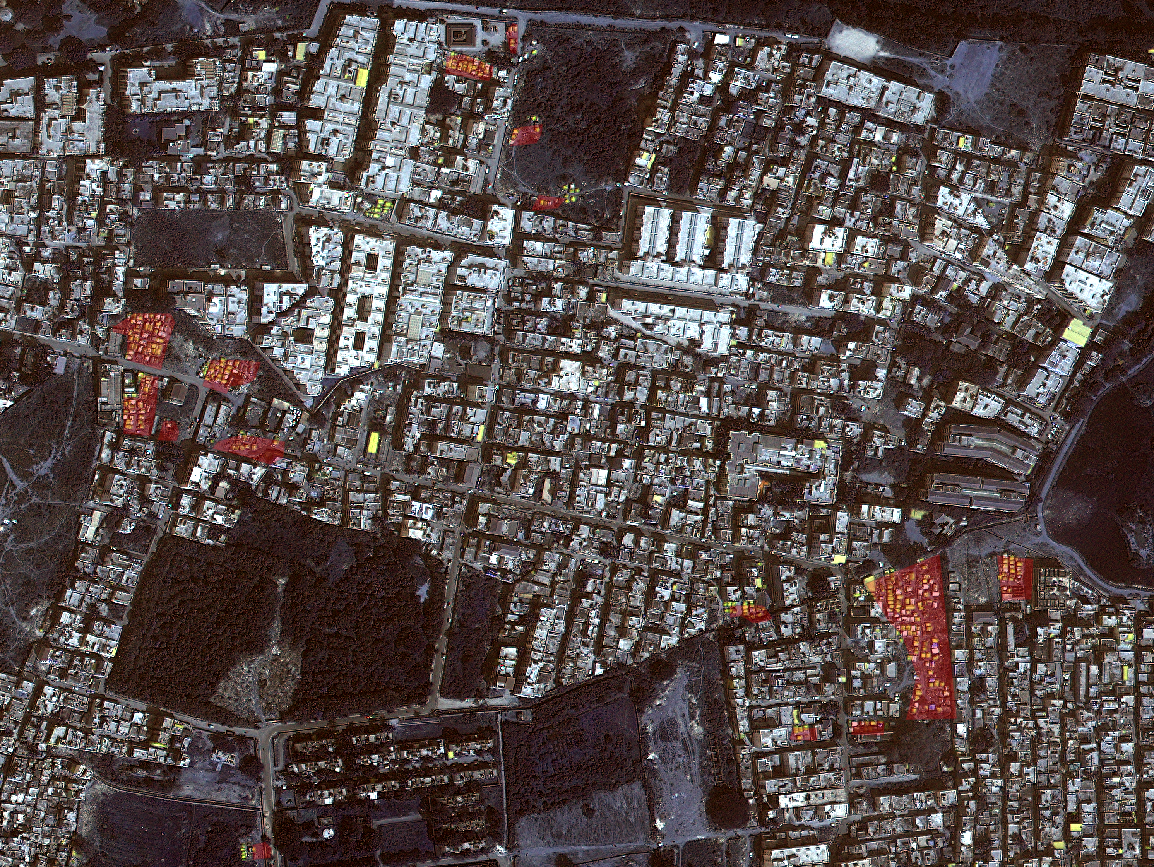
\includegraphics[width=\linewidth]{images/section_3}
%  \caption{Dense informal area in Bangalore, the red patches indicate informal
%  settlements}
%  \label{fig:section_3}
%\end{figure}

\begin{figure}
\centering
\begin{tabular}{cc}
  \subfloat[Section 1]{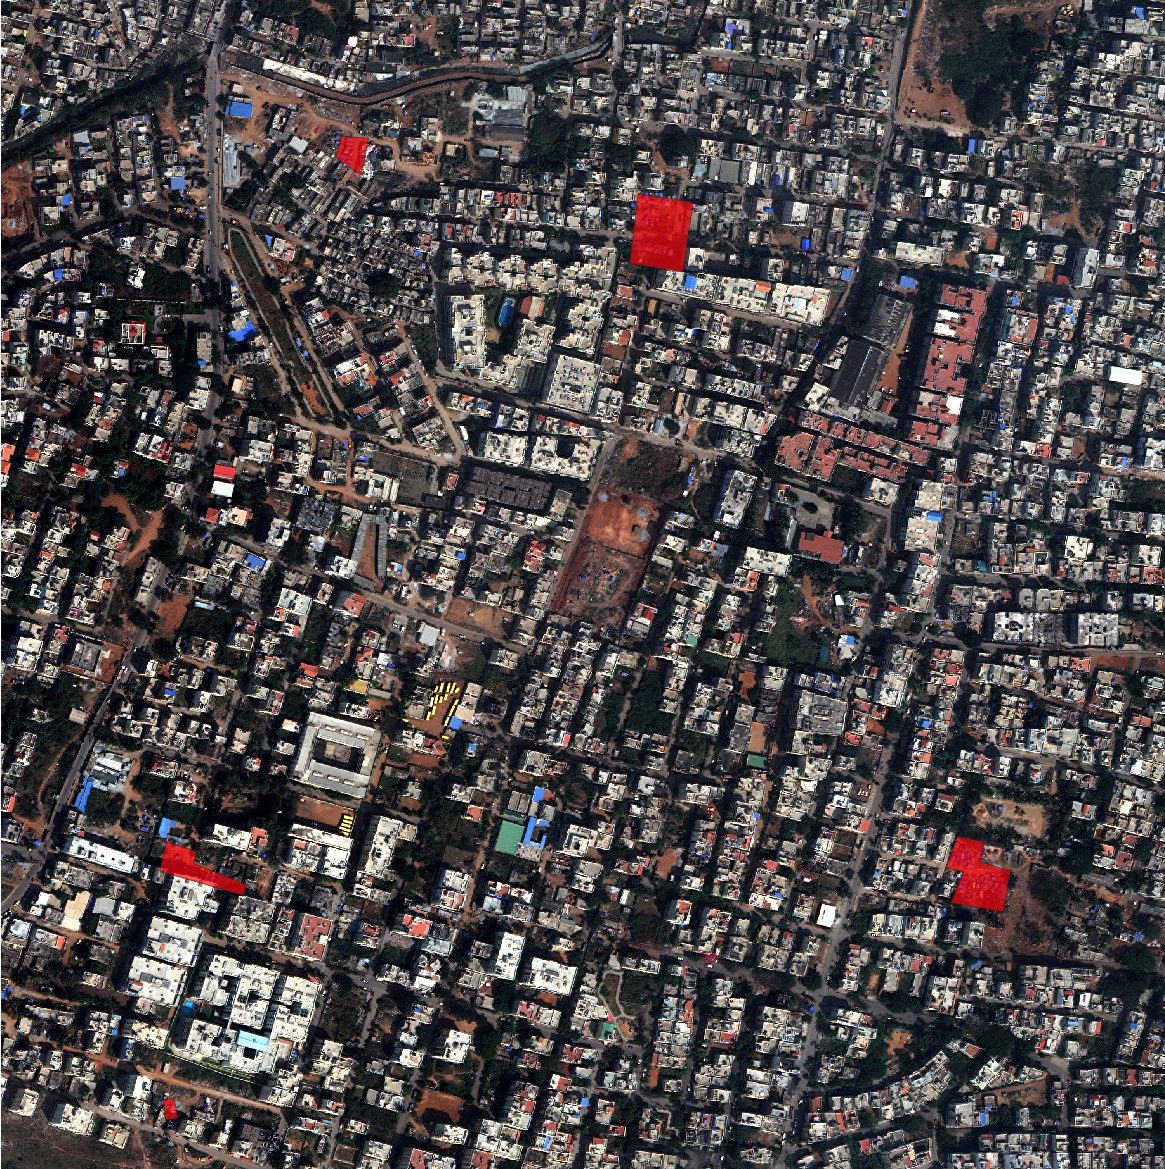
\includegraphics[width=6.2cm, height=5cm]{images/section_1_gt}}&
  \subfloat[Section 2]{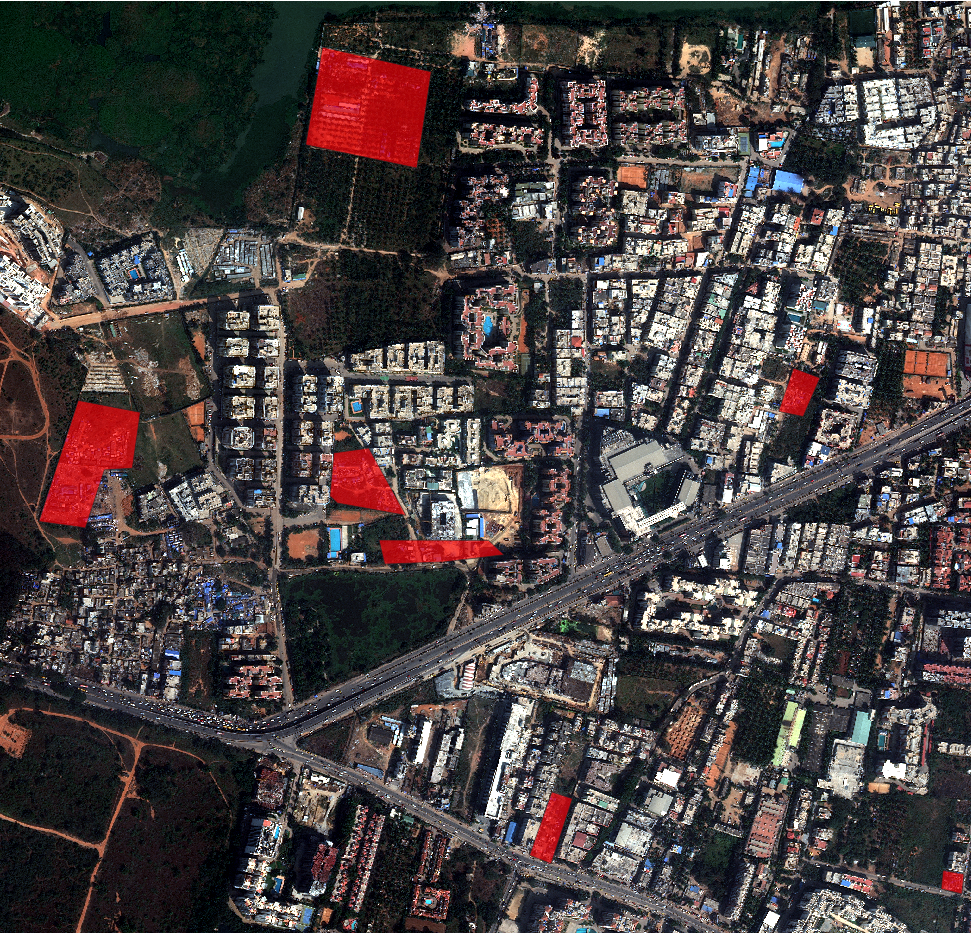
\includegraphics[width=6.2cm, height=5cm]{images/section_2_gt}}\\
  \subfloat[Section 3]{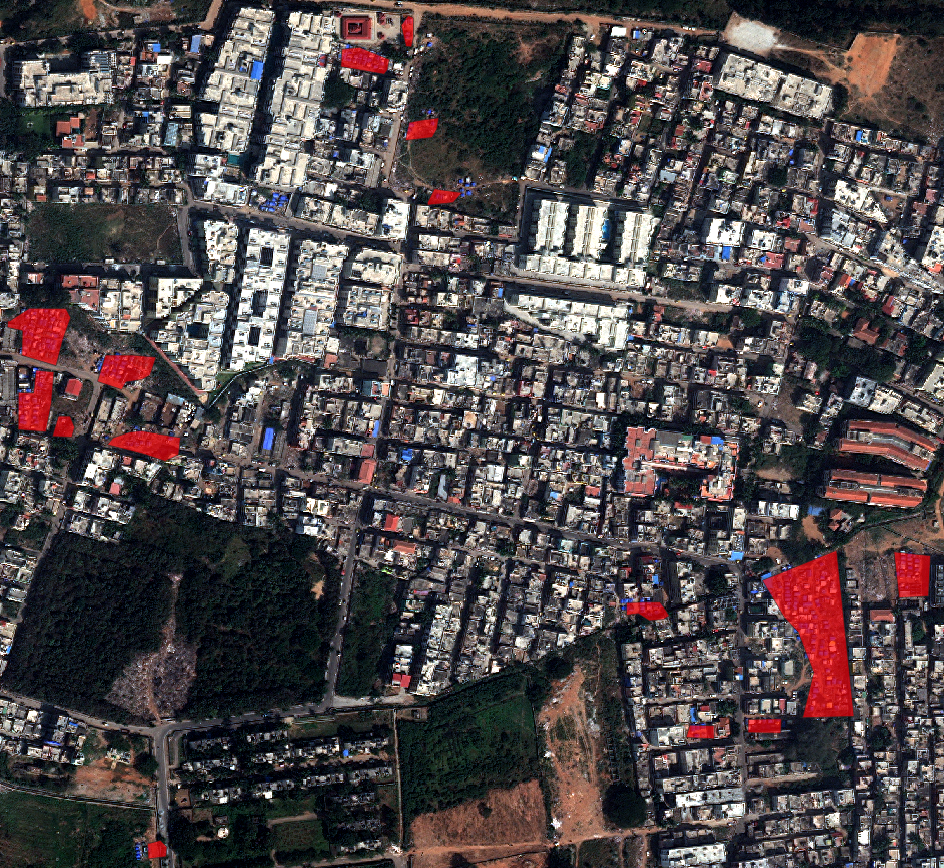
\includegraphics[width=6.2cm, height=5cm]{images/section_3_gt}}&
  \subfloat[Location of Sections]{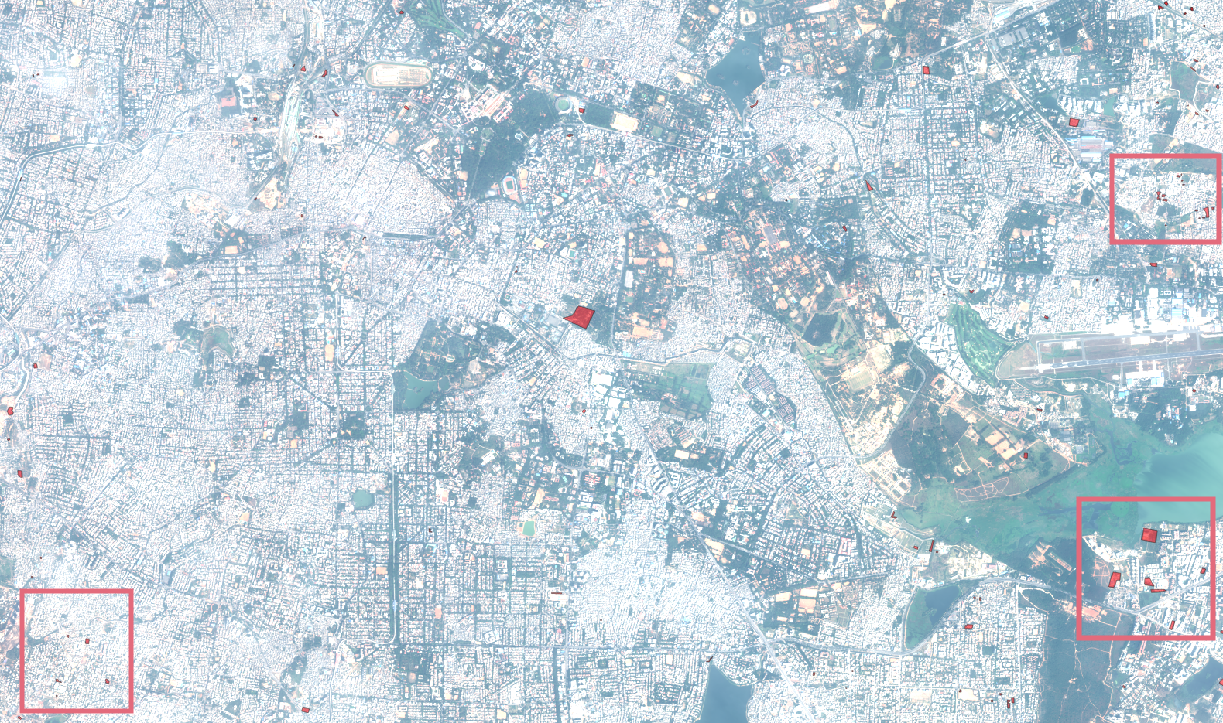
\includegraphics[width=6.2cm]{images/west-bangalore_sections}}
\end{tabular}
\caption{The images used for evaluation and classification}
\label{fig:sections}
\end{figure}



\section{Conventional Feature Extraction Methods}
Studies often use a combination of features in the detection of informal settlements. Our research will use methods for feature extraction that performed well in previous research \cite{graesser2012image}. The methods we use are the Histogram of Oriented Gradients (HoG) and Line Support Region (LSR) features. Both HoG and LSR are already implemented in a Python library. This library, called spfeas, that is based on the research Graesser \textit{et al.} conducted on the classification of formal and informal neighborhoods \cite{graesser2012image}. Besides these two features we design a new method that measures the difference 
in prevalence and distribution of road intersections between formal and informal areas. This is based on the belief that there is a difference in this aspect between formal and informal areas.

\subsection{Terminology}
The paper of Graesser \textit{et al.} \cite{graesser2012image} uses blocks of pixels instead of each individual pixel when extracting features from images.  This is to ease the computational load because the extraction methods used are
computationally quite expensive, especially LSR. These blocks of pixels are of 20 by
20 pixels in the paper. The size of these pixel blocks is referred to as the \textit{block size}. In our research, the block size will differ from
this value to evaluate the affect to the performance of the features.
In addition to blocks, the paper also uses a set of different scales for the
calculation of features. A scale specifies the pixels around a block that
are used for the calculation of that block. This allows blocks to be
spatially connected to the surrounding areas, which can increase the
performance of features.

\subsection{Histogram of Oriented Gradients}
% designed for only settlement detection
% as supporting feature
% theory part
% however, Graesser does work for differentiating
% picture for explaination?


The Histogram of Oriented Gradients was originally used for the detection of
man-made structures in images. The features retrieved from the histogram were
able to differentiate between natural and man-made sections in an image. This
approach of man-made structure detection relies on the difference in the
distrubution of gradients in a particular region of the image. Because man-made
structures are often consists of straight lines and regular forms, this
contrasts the irregular forms that are naturally formed. This difference in
appearance translates to a difference in the distribution of gradients in
man-made structures and nature.

In satellite images, the difference of the Histogram of Oriented Gradients
between nature and human settlements is quite large. Eventhough HoG was
originallly used for differentiating between nature and man-made structures,
the paper of Graesser et al was able to succesfully to use HoG between formal
and informal neighborhoods. The paper uses the disparate spatial distribution of
buildings in formal and informal regions. The
placement of houses in formal regions are often placed in a regular pattern
with fixed orientations. Informal areas, in contrast, are usually constructed
without a design or regular pattern. This difference in regularity is
a characteristic that can be used for classification of formal or informal
settlements.

The order of regularity of an area can be captured using the number of
orientations in which buildings are constructed. Few distinct orientations suggest
a formal settlements while many orientations suggest informal. The orientations
of buildings are calculated using the gradients returned by the application of
a binary filter on the image. The gradients are quantized into a set of
orientations or bins. This results in a histogram commonly named the Histogram
of Oriented Gradients. High peaks in the HoG correspond to a multitude of
similar gradients, thus uniformity in the image. Since uniformity is linked
to formal settlements, high peaks in the histogram correlate with formal
settlements. The informal settlements, on the other hand, are characterized by
the absence of peaks in the HoG due to the multitude of different gradients
caused by the irregular placement of buildings.

Applied in practice, the paper from Graesser et al extracts five
characteristics from the HoG: two types of mean, variance, skew, and
kurtosis. These properties of the histogram are used as features to
describe the histogram and differentiate between formal and informal regions.
These 5 features will be calculated for every color band of the image,
resulting in a grand total of 15 features for the Histogram of Gradients.
According to the results presented in the paper, these 15 features alone could
result in an accuracy of 65 to 75 percent. It must be noted, however, that this feature was applied to specific regions where the visual difference between formal and informal was substantial, which is often not the case.

\subsection{Line Support Region Features}

The formality of regions can be for a part be determined by observing the
spatial distribution of neighborhoods. In the same manner as HoG characterized
areas by the orientation their buildings, neighborhoods, alternatively, can be
characterized by the size of their buildings. Informal settlements generally
lack the presence of large buildings in contrast with formal regions. The size
of constructions can be characterized using the Line Support Region (LSR)
features \cite{unsalan2004classifying}. Likewise to HoG, LSR utilizes gradients
calculated from remote sensing imagery. LSR uses the fact that straight lines
have uniform gradients. In practice, natural photographs hardly contain
perfectly straight lines, which results in similar but non uniform gradients of
lines. Therefore, LSR uses groups similar gradients to represent a line in
images to detect semi straight lines in images \cite{burns1986extracting}.

The LSR is implemented in spfeas in accordance to the paper of Graesser \textit{et al.} \cite{graesser2012image}. The paper uses three statistical features extracted
from the LSR, these are: line length entropy, mean, and entropy of line
contrasts. Together with three color bands, this brings the total to nine
features for a single scale. Using only LSR features and scales 50, 100, and 200, the paper achieved an accuracy of 60 to 75 percent.


\section{Road Intersection Density}

In this field of study, as we have discussed, there exist many methods for characterizing image regions on land use. In some of these methods, the road network is used to try to classify regions, for instance, using road accessability metrics \cite{owen2013approach}. Using the road network to classify between different types of land use seems a promising approach to detect slums. We aim to extract the properties of the road network using a new strategy by detecting the road intersections in the image. This is based on the hypothesis that the density of the road intersections translates to the density of the road network, which is different for various types of neighborhoods. In our case, slums are visually and spatially distinct from surrounding building types, which could infer a difference in the road network density. Extracting density from the road intersections might therefore allow us to differentiate slums from their surroundings. In the next sections, we will discuss the various approaches we have used in the extraction of intersections for satellite images.



\subsection{Convolutional Neural Network}

Road detection and extraction from satellite images is well established field of study with a large variety of developed methods \cite{mena2003state}.  The specific detection of road intersection is less studied although there are studies covering the subject \cite{hu2007road} \cite{koutaki2004automatic} as part of general road network extraction. Since there exists a base of research in this field, we can use established methods to extract the road network, which can consequently be used as a basis for the extraction of the road intersections. 
A promising approach in road extraction is the use of Neural Networks \cite{mangala2011extraction} \cite{mokhtarzade2007road}. A study from 2017 was able to extract both the road network together with buildings with high accuracy using a Convolutional Neural Network \cite{alshehhi2017simultaneous}. We used the same approach although with a separate implementation of the convolutional neural network since the research paper did not include the software and data that was used in the study \cite{airs}. This implementation included a open-source set of images, that was designed for the training and validation of the neural network \cite{MnihThesis}. After training on the provided images, the network was tested on our own satellite images, resulting in erroneous predictions as it did not represent the road network in the provided image. The suspected cause of this failure is the difference in the training data to our satellite imagery data. The trainingset that was used contained satellite images obtained from mostly rural area's of the state of Massachusetts in the United States, while the data used in our research is from Bangalore in India which is mostly urban. The geographical features and the road systems presented in the two locations appears to be rather different, which could be a probable cause for the inability of the neural network to recognize the road network in Bangalore. Furthermore, the difference in resolutions of the two image sets could be another cause as the images of Massachusetts were of quite a lower resolution than the images of Bangalore.

\subsection{Hough Transform}
As an alternative to the neural network, we attempted to extract road networks using image processing techniques, which uses a number of operations resulting in a prediction of the road network. The first operation is the transformation of the RGB image to grayscale values, which is in preparation for Otsu's method for threshold, which is able to separate buildings from roads \cite{otsu1979threshold}. The resulting image, displayed in Figure \ref{fig:roads_hough}, is the predicted road network in the satellite image, where the white regions are detected as road. 

From an aerial point of view, the properties of roads are often elongated thin lines with constant width, and are often not possessed by other types of structures in images. We therefore detect these lines as roads using a Hough transform, which is able to extract straight lines from images and create mathematical definition of the lines \cite{duda1972use}. Once the roads are mathematically defined, determining the location of the intersection is straightforward.

\begin{figure}
\begin{tabular}{cc}
  \subfloat{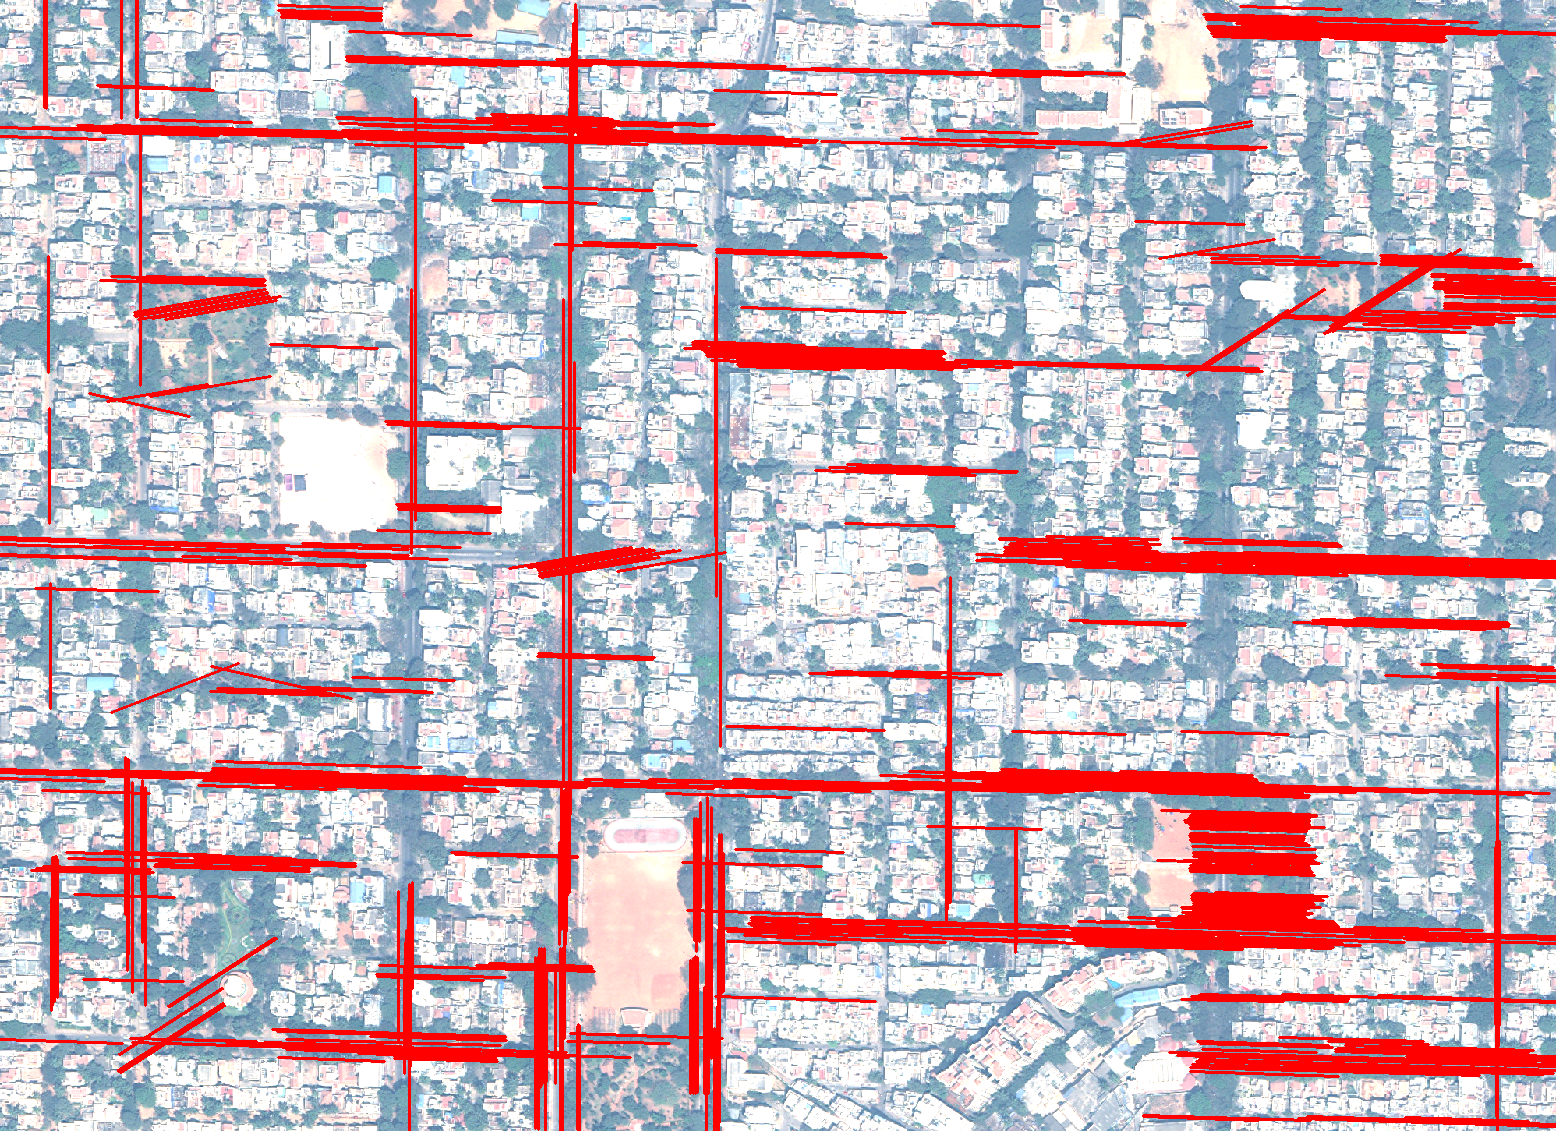
\includegraphics[width=7cm]{images/hough_road_section_8}}&
  \subfloat{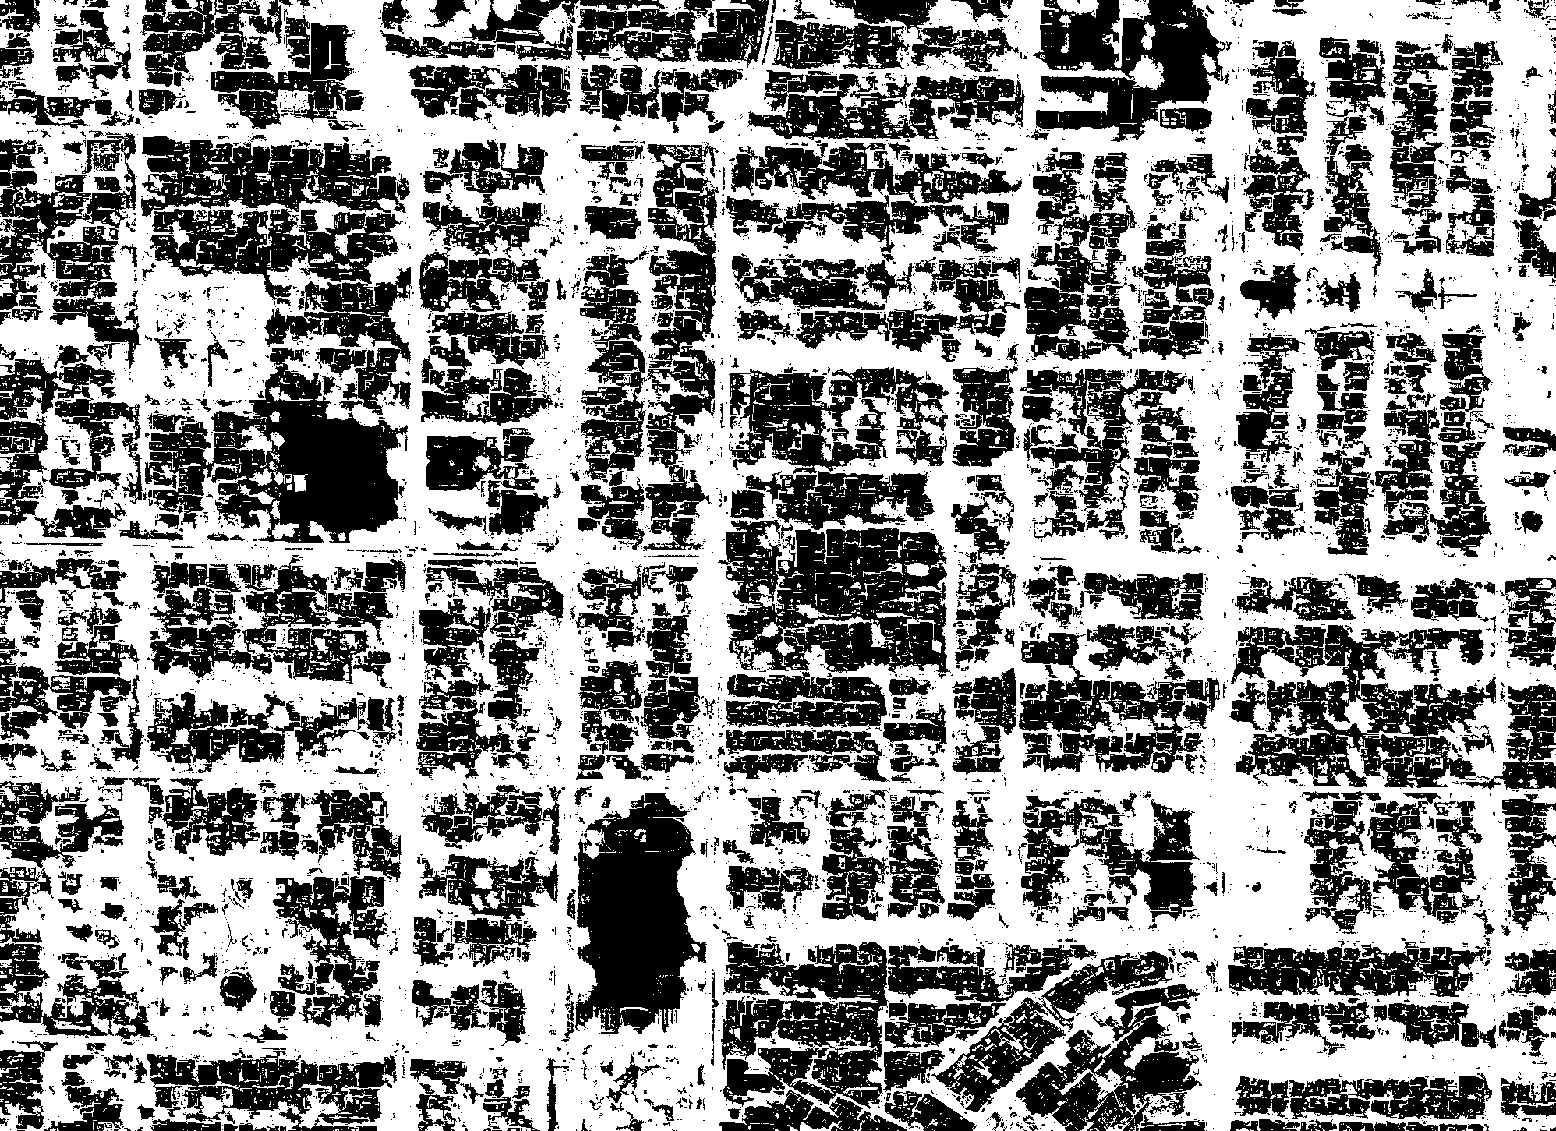
\includegraphics[width=7cm]{images/hough_road_section_8_mask}}
\end{tabular}
\caption{Detected roads using Otsu's thresholding method (left) combined with
Hough Transform (right)}
\label{fig:roads_hough}
\end{figure}

This method for road intersection detection was implemented in Python, resulting in a predicted road network and detected Hough lines displayed in Figure \ref{fig:roads_hough}. This was the most balanced results were able to achieve after changing the parameters for the creation of the prediction mask and Hough lines; different parameters would drastically increase recall and decrease accuracy beyond useful application. In this case, in contrast to the neural network, the extracted mask represents the road network quite accurately although the hough transform resulted in a lot of duplicate lines and noise. Even though the noise might be filtered out, we decided to pursuit a different method of intersection extraction. 

\subsection{Road Intersection Convolution}
In contrast to the original approach that first extracts the road network followed with the to detection of the intersections, we changed the approach of intersection detection to directly extract intersections from the satellite image. In our new approach, we apply a convolution using a kernel in the shape of an cross directly on the satellite image. Because the kernel matches the shape of an intersection, the output of the convolution will have peaks in the output image on the positions of the intersections. The results from the proof of concept are displayed in Figure \ref{fig:roads_conv}.
This approach is partly based on previous research; it has similarities to the use footprints to find the direction of intersections \cite{hu2007road}. The footprint approach uses certain points, called seeds, in the image from where the road network expands using road segments. These road segments can be one of a few classes, for example, a straight road, T junction and cross intersection. The type depends on its surrounding pixels, which form a footprint that is classified as either one of the listed classes. Another study used a similar approach, which explicitly displays the different sizes of intersections \cite{koutaki2004automatic}. However, these two studies do not use convolution but different methods to match the footprints to the intersections in the image. Our method does not have to be as complicated because the orientation of an intersection is not important in our case, only the location is required.

\begin{figure}
	\begin{tabular}{cc}
		\subfloat{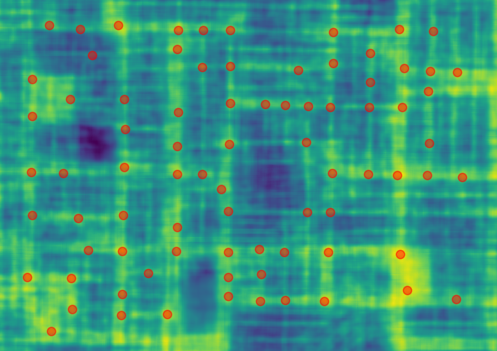
\includegraphics[width=7cm]{images/conv_road_section_8_1}}&
		\subfloat{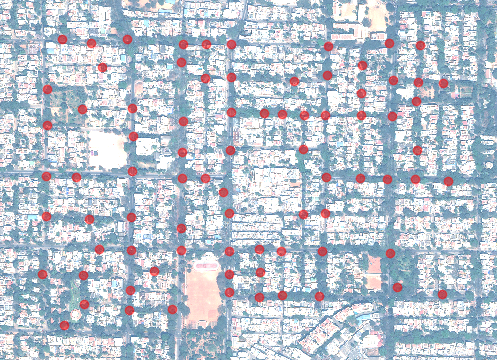
\includegraphics[width=7cm]{images/conv_road_section_8_2}}
	\end{tabular}
	\caption{Detection of intersections using convolution of a cross shaped kernel.
		Left: Heatmap of output of the convolution; Right: Located peaks overlayed on input image}
	\label{fig:roads_conv}
\end{figure}

Preceding the convolution, the satellite image is transformed to grayscale and subsequently inverted in color. In certain areas, the grayscale version of the image will already have a large contrast between roads and the surrounding buildings. However, this not true for the sections displayed in Figure \ref{fig:sections}. We therefore apply the Otsu's thresholding is after the transformation to grayscale, which results in a black and white version of the image with a large contrast between roads and buildings. 

The original kernel that was used as proof of concept is a n by n matrix, containing a cross of ones
with the remainder filled with zero's, as illustrated in Figure \ref{fig:conv_kernel}a on the left. To clarify some terminology, the toe of an intersection is one of the roads leading to the
intersection. In the case of Figure \ref{fig:conv_kernel}a, there are four toes
with a width and length two and three matrix cells, respectively. The width and length of a toe will also be referred to as the road width and length respectively. Theoretically, this kernel has the optimal activation when it is exactly placed on the same shape of the kernel, thus the shape of a cross intersection. It is therefore important to match the shape of the kernel to the shape of the intersections in the image, which means that the width of the toe in the kernel depends on the road width of the intersections in the image. Therefore, the dimension of the kernel depends on the image used and the scale of the image. In practice, the kernel will be much larger than the kernel in Figure \ref{fig:conv_kernel}a as the road width and length are generally in the dozens rather than the single digits.

\begin{figure}%	
	\centering
	\begin{tabular}{cc}	
		{$\displaystyle
			\begin{pmatrix}
			0 & 0 & 0 & 1 & 1 & 0 & 0 & 0\\
			0 & 0 & 0 & 1 & 1 & 0 & 0 & 0\\
			0 & 0 & 0 & 1 & 1 & 0 & 0 & 0\\
			1 & 1 & 1 & 1 & 1 & 1 & 1 & 1\\
			1 & 1 & 1 & 1 & 1 & 1 & 1 & 1\\
			0 & 0 & 0 & 1 & 1 & 0 & 0 & 0\\
			0 & 0 & 0 & 1 & 1 & 0 & 0 & 0\\
			0 & 0 & 0 & 1 & 1 & 0 & 0 & 0
			\end{pmatrix}
			$} &
		$\vcenter{\hbox{
\includegraphics[width=4cm]{images/gauss_kernel}}}$\\
		a) Simple convolution kernel & b) Gaussian convolution kernel
	\end{tabular}
	
	\caption{Different convolution kernels}%
	\label{fig:conv_kernel}
\end{figure}

Figure \ref{fig:roads_conv} displays the results of the convolution and the corresponding location of the detected peaks. The image used was a small section of the satellite image of Bangalore, not to be confused with the other three sections. This specific region was chosen because of the width of the roads and the regularity of the road network with 90 degree angles between the toes of the intersection. Furthermore, the horizontal and vertical roads run parallel to the edges of the image. The road network is also quite distinct from the background despite the vegetation covering large part of the roads, which might actually increase the contrast between the road and the surroundings.

The peaks, displayed as red dots, are located using local maxima detection from the Python scikit-image package \cite{scikit-image}. This function detects local maxima in an image, which are regions that stand out from surrounding values. 

\subsubsection{Kernels}
In the development of this method, we have designed a number of kernels to extract road intersections from images. In order to increase accuracy of the detected intersections, we created a new type of kernel that is similar to the kernel displayed in Figure \ref{fig:conv_kernel}a, but with the zero's replaced by negative numbers. The distance from the cross is proportional to the negative value of a cell in the kernel. When applied to areas which are not an intersection, the negative cells of the kernel should produce a large negative activation. In practice, this kernel seems to be activated by intersection as well as straight sections of road, which introduces many false positives.

To account for different widths of roads in an image, we created a kernel using Gaussian distributions, displayed in Figure \ref{fig:conv_kernel}b. This kernel should smooth the contrast between roads and roadside and might remove noise. This kernel counts the center of the road the most while the edges
of the road count for less. This should increase the scalability of the kernel to multiple types and sizes of roads, such as alleys or main streets. The Gaussian kernel will therefore used for experiments on the three image sections.

\subsubsection{Intersection Detection Evaluation}

\begin{figure}
\begin{tabular}{cc}
  \subfloat{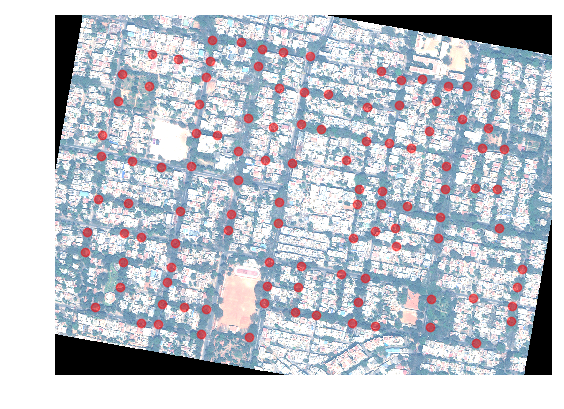
\includegraphics[width=7cm]{images/rot10}}&
  \subfloat{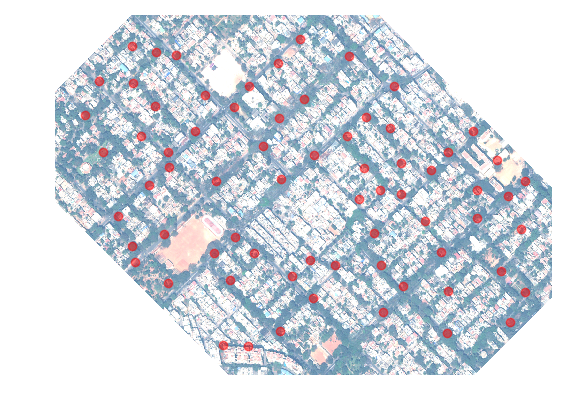
\includegraphics[width=7cm]{images/rot45}}
\end{tabular}
\caption{Performance of intersection detection in rotated intersections, from
  left to right with 10 and 45 degrees respectively}
\label{fig:roads_rot}
\end{figure}

A fundamental problem of this approach is the relation between the kernel and the resolution of the image. An increase of the scale or resolution of an image will change the dimensions of the intersections, thus requiring a change to the content of the kernel. Although the Gaussian distribution should increase scalability, it is still largely required to adjust parameters according to the resolution of the image.\newline

\noindent
Because of the fixed orientation of the cross in the kernel, this approach should inherently be prone to differences in orientation. In the proof of concept, we explicitly used a road system with a constant orientation, as displayed in Figure \ref{fig:roads_conv}. The constant orientation of the intersections, enable the kernel to correctly detect a large number of intersections. In many other areas, the road system is not nearly as consistent, for instance ,the sections displayed in Figure \ref{fig:sections}. Intersections that are rotated relative to the orientation of the kernel should therefore be more difficult to detect. To test this hypothesis, we performed the intersection detection under rotations of 10 and 45 degrees, as displayed in Figure \ref{fig:roads_rot}. It seems that, under slight rotation, the fast majority of intersections are still detected whereas increasing the rotation to the maximum of 45 degrees results in a loss of many detections. Interestingly enough, there is almost no increase in false positives. It might be that this seemingly invariance to rotation is caused by the method of peaks detection.  When using a rotated image, the resulting convolution is more smooth with less peaks compared to the original image. It seems that the local maxima detection is still able to correctly detect these faint peaks in the convoluted image. Nevertheless, this approach should primarilty be used for images with minimal rotation since this produces the most correct detections.\newline

\noindent
The road system displayed in figures \ref{fig:roads_conv} and \ref{fig:roads_rot} do not well represent the general road network encountered in the whole of the satellite image. This becomes apparent when observing the road system in the three section displayed in Figure \ref{fig:sections}. Although the majority of land area in these sections is formal, there is a clear contrast between these road systems and the road system used in the development of this feature. The road system in the three sections are much more narrow, shorter, and less regular than the road system in \ref{fig:roads_conv}. In these sections, on many occasions, even manual extraction of intersections is quite difficult. It is, for instance, often not clear whether the space between two buildings is an empty strip of land or actually a road. 

%Due to the different nature of the road systems, parameters used to detect the intersections in Figure \ref{fig:roads_conv} and the sections in Figure \ref{fig:sections} are different. Because the streets in these three sections are generally more narrow and less long, both the road width and road length parameters are decreased relative to the parameters used in Figure \ref{fig:roads_conv}. Furthermore, the parameters for the local maxima detection are changed to only detect peaks that are really distinct from their surroundings. The motivation behind this is to reduce noise introduced by the irregularity and obscurity of the road network.

We could not perform a objective evaluation of the intersection detection due to the lack of a ground truth of the road intersections. Since we are not in the possession of a ground truth, we cannot calculate objective measures of detection performance, such as accuracy, recall and the F1 score. Instead, the performance evaluation of the various methods and parameters used for the detection of intersection is based on visual observation.

In conclusion, the use of a cross shaped kernel together with convolution seems to be able to extract the location of road intersections quite well. Although, for real world applications, such as road system mapping, this method for intersection detection might not be sophisticated enough, since this method does not include the direction of the intersection. Furthermore, false positives and negatives are quite prevalent using this approach; it might meet not the performance achieved by different methods.

\subsection{Feature extraction}

\begin{figure}
	\begin{tabular}{cc}
		\subfloat{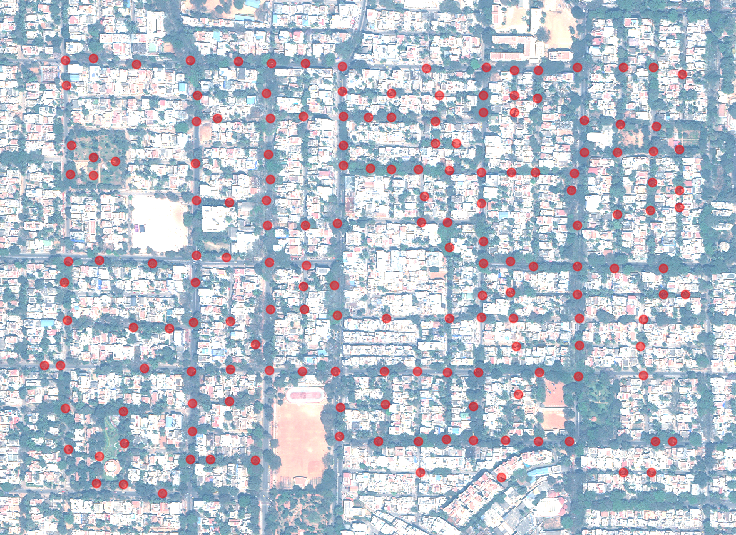
\includegraphics[width=7cm]{images/hotspotint}}&
		\subfloat{
\includegraphics[width=7cm]{images/hotspot}}
	\end{tabular}
	\caption{Hotspots extracted from the detected intersections. Left: Detected road intersections; Right: Resulting hotspot map of the local G function}
	\label{fig:roads_hotspot}
\end{figure}


The positions of the road intersections extracted from the image are used to create a intersection density map of the area. The density of road intersections in an area is measured using spatial statistics provided by the Getis and Ord's local G function \cite{getis1992analysis}. The local G function is a measure of spatial association between spatially distributed data. In our case, this data is the locations of the intersections in the image. The local G function is able to detect local hotspots and coldspots in instance data, effectively indicating the location of hotspots and coldspots in the density of intersections in the image of interest.

\begin{figure}[h]
	\centering
	$ \mathlarger{\mathlarger{\mathlarger{ G_i(d) = \frac{\sum\limits_{j=1}^{n}w_{ij}(d)x_j}{\sum\limits_{j=1}^{n}x_j} }}} $
	\caption{Definition of the local G function}
	\label{g_function}
\end{figure}


The formula of the Getis-Ord local G function $G_i(d)$ is displayed in Figure \ref{g_function}, which defines for a data point $i$ on a Cartesian plane a ratio using the neighboring data points within a radius $d$. In our case, $i$ is the location of an intersection, with $d$ being the scale of the feature. Regarding the variables in the numerator of the fraction, $n$ is the total number of data points, $j$ is every data point that is not $i$, $w_ij{d}$ is a function that returns zero or one whether $j$ is within the radius $d$ of $i$, and $x_j$ specifies the weight of $j$. The enumerator sums up all weights $x_j$ of the data points within the radius $d$ of $i$. In our case, when using the location of road intersections, we do not have weights other than ones. However, because we rasterize the locations of the intersections to a grid in the shape of the HoG and LSR features, the weights will indicate the number of intersections that fell within a certain block in the grid. The denominator is the sum of the weights of all data points, regardless of their location. This fraction is in essence a ratio between the points within the radius of $i$ and all points. 

\begin{figure}[h]
	\centering
	$ \mathlarger{\mathlarger{\mathlarger{ z = \frac{x - \mu}{\sigma} }}} $
	\caption{Definition of the Z score}
	\label{z_score}
\end{figure}

We use the ratios created by $G_i(d)$ to create a statistical feature using the Z score. This score is calculated using the formula displayed in Figure \ref{z_score} where $x$ is the $G_i(d)$, $\mu$ is the mean and $\sigma$ the standard deviation of all $G_i(d)$ \cite{kreyszig2010advanced}. The Z score is a form of outlier detection, where negative and positive scores indicate a deviation from the mean. Using the Z score, we can detect hot and cold spots in the $G_i(d)$ ratios, and therefore detect hotspots and cold spots in the density of road intersections. The exact calculation of the Z score for the local G function with definitions of the $G_i(d)$ mean and variance can be found in the paper\cite{getis1992analysis}. The Z score applied to local G function results in a map of hotspots and cold spots of the road intersections, as illustrated by Figure \ref{fig:roads_hotspot}.

Both the local G function and Z score are implemented in the PySal Python packackage \cite{rey2010pysal}. The resulting map from the local G function and Z score is used as a feature and will be referred to as the \textit{Road Intersection Density} or RID for short.







\section{Feature Evaluation}

In order produce a functioning classifier, the predictive value of the features
must be evaluated. This assesses wether a certain feature is useful in the
discrimination between formal and informal. The evaluation requires the
knowledge of what parts in a satellite image are formal and informal to create
a distinction between the two classes. This knowledge is represented in
a ground truth, this is a mask covering the satellite image indicating the
informal regions.

The mask is used to divide each block of pixels into the two classes, formal
and informal. Each block has a vector of values, also called features,
characterizing that particular block. Because the blocks are grouped together,
the features associated with the same class are grouped together as well. This
allows for the analysis of the distribution of the features in both classes. If
the distribution of a certain feature varies quite distinctly between the two
classes, this indicates as a suitable candidate for classification of informal
regions.

The groundtruth mask is constructed using a vector file containing the
boundaries of informal areas. The boundary file is rasterized and applied on
top of the satellite image, creating a mask of the informal settlements.
Because classification and feature calculation is performed on blocks instead
of pixels, the pixel based mask transformed into a block based mask. In this
mask, every pixel represents a block where the zero represents formal and one
represents informal. This effectively creates a ground truth.  

The predictive value of a feature can be visualized using a boxplot of the two
classes. When a feature is distinctive on its own, the distribution of the
values in the two classes will be different. The data used for the evaluation
comes from three small sections of the image. As priorly mentioned, this
creates a more even division of classes which should provide a more accurate
evaluation of the selected feature.

The features will be calculated for every image at different block sizes and
scales. Because block size and scale impact the predictiveness of a feature,
various combinations are used to discover the most favorable combination.

% TODO: insert concatenated image of the three sections

%Eventhough there might not be
%a significant difference between two distribution, by using multiple features
%in combination, the grand total might more distinctive that the sum of its
%parts. 

\subsection{Histogram of Oriented Gradients}

In the analysis of the historgram used block sizes of 20, 40, and 60 combined
with scales of 50, 100, 150, and 200. These combinations should capture the
difference that either an increase of block size or scale causes to the
predictiveness of a feature. For visualization purposes, only a single feature
of the 15 features of HoG of a single section is displayed here. This feature
is the most distinct between formal and informal. The other two sections are
comparable to the section used here. Moreover, not all combinations of the
block sizes and scales are presented here, only a few examples which illustrate
the distinctiveness of the features of the Histogram of Oriented Gradients.

\begin{figure}
\begin{tabular}{cc}
  \subfloat{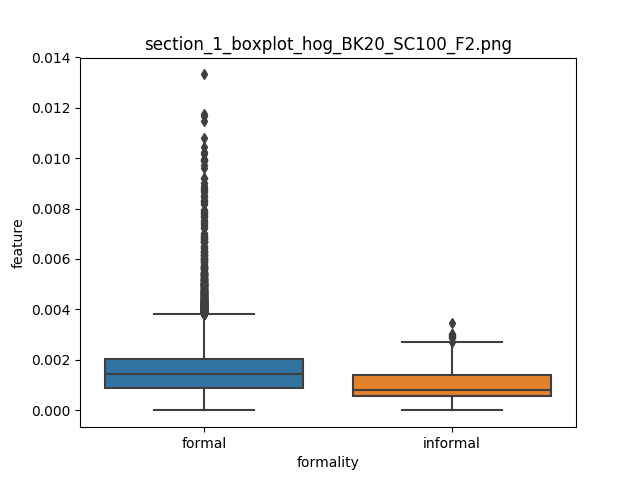
\includegraphics[width=4cm]{images/HoG/inc_bk/section_1_boxplot_hog_BK20_SC100_F2}}&
  \subfloat{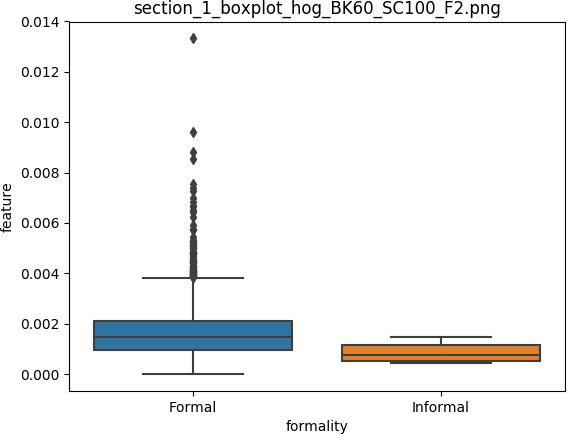
\includegraphics[width=4cm]{images/HoG/inc_bk/section_1_boxplot_hog_BK60_SC100_F2}}\\ 
  \subfloat{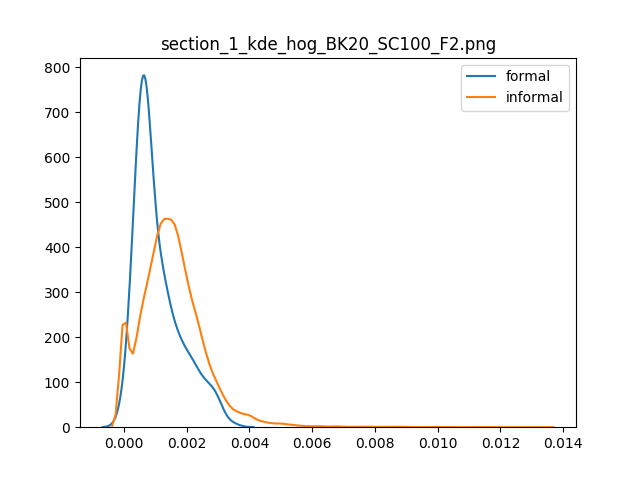
\includegraphics[width=4cm]{images/HoG/inc_bk/section_1_kde_hog_BK20_SC100_F2}}&
  \subfloat{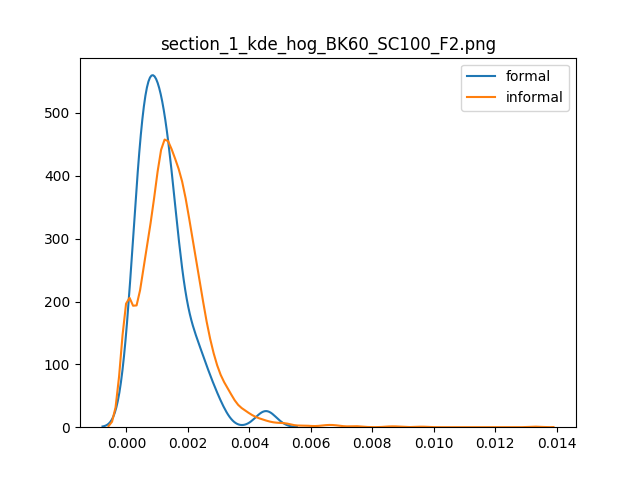
\includegraphics[width=4cm]{images/HoG/inc_bk/section_1_kde_hog_BK60_SC100_F2}}
\end{tabular}
\caption{The effect of increased block size on a HoG feature. From left to
right: a block size of 20 and 60 respectively.}
\label{hog_inc_bk}
\end{figure}

Figure \ref{hog_inc_bk} shows the effect that an increased block size has on
the distribution of values in both classes. This example uses a constant scale
of 100 pixels and a variable block size of 20 and 60 pixels. The experiment
with a block size of 40 is performed as well, but is ommited from the figure to
keep the results brief. A more comprehensive visualization of the evaluation
can be found in the appendix. It seems that the block size, in this case, does
not influence the both distrutions significantly. As a result an increase in
the size of a block will have little influence on the predictive value of the
HoG.

\begin{figure}
\begin{tabular}{cc}
  \subfloat{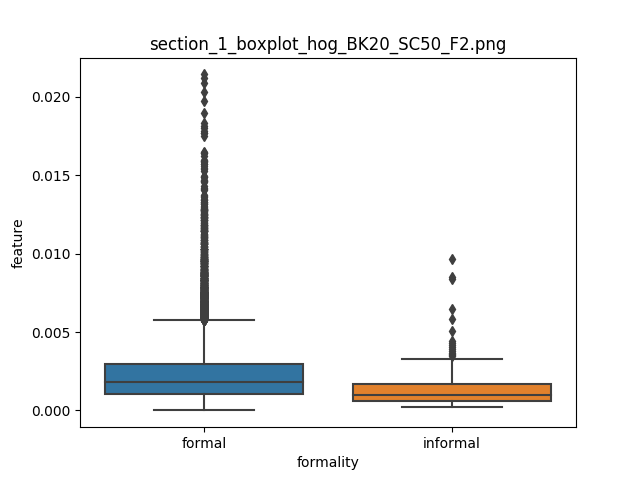
\includegraphics[width=4cm]{images/HoG/inc_sc/section_1_boxplot_hog_BK20_SC50_F2}}&
  \subfloat{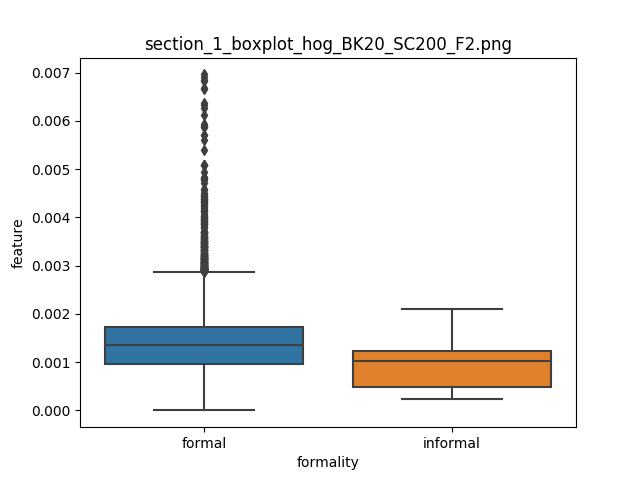
\includegraphics[width=4cm]{images/HoG/inc_sc/section_1_boxplot_hog_BK20_SC200_F2}}\\
  \subfloat{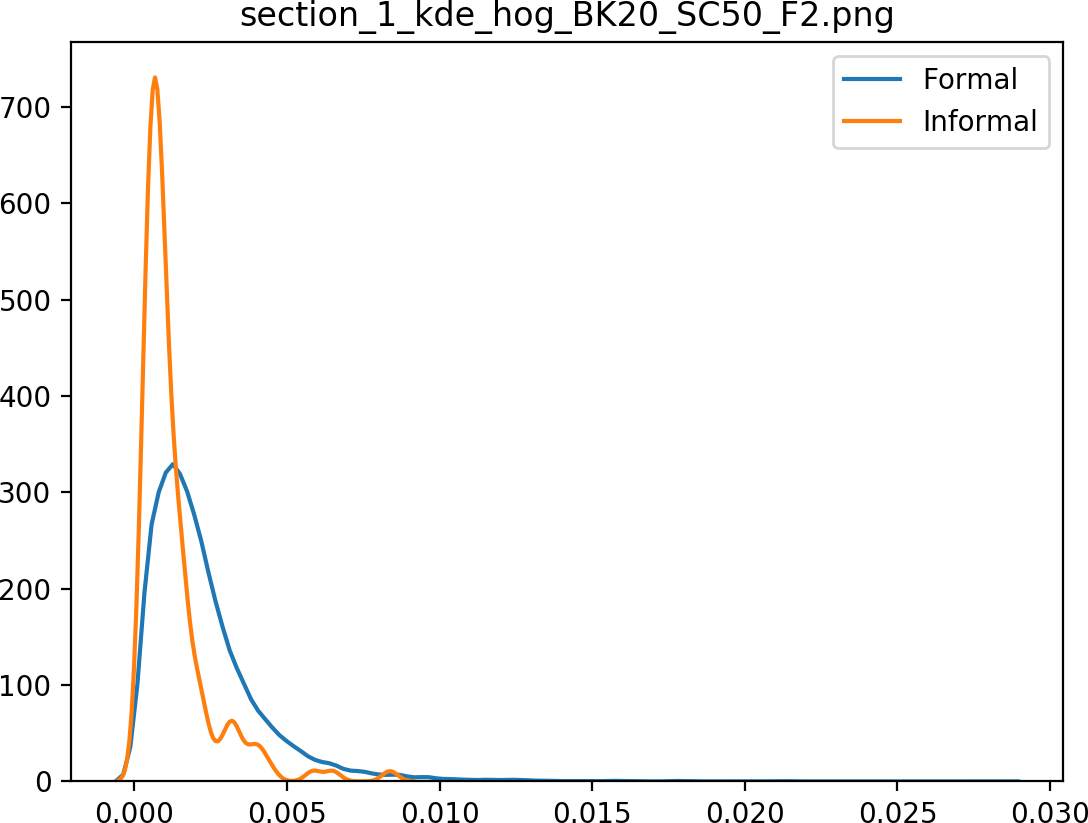
\includegraphics[width=4cm]{images/HoG/inc_sc/section_1_kde_hog_BK20_SC50_F2}}&
  \subfloat{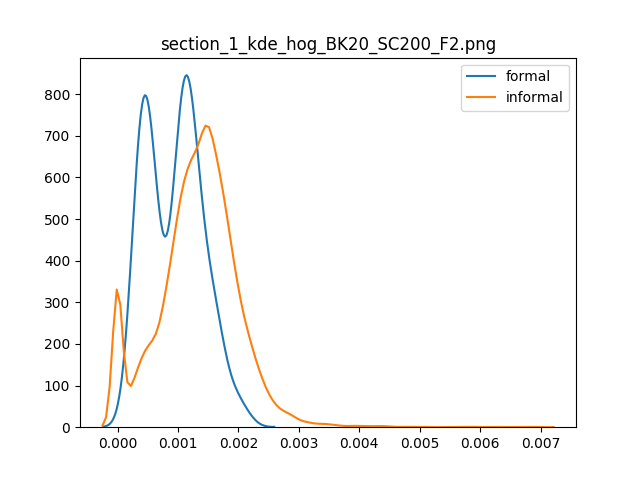
\includegraphics[width=4cm]{images/HoG/inc_sc/section_1_kde_hog_BK20_SC200_F2}}\\
\end{tabular}
\caption{The effect of increased scale on a HoG feature. From left to
right: a scale of 50 and 200 respectively}
\label{hog_inc_sc}
\end{figure}

Figure \ref{hog_inc_sc} illustrates the effect of increased scale on a constant
block size. It seems to indicate that an increased scale leads to an increased
separatation of the two distribution, thus increasing the predictiveness of the
feature.

\subsection{Line Support Region}

Similar to the analysis of the Histogram of Oriented Gradients, the analysis of
Line Support Region uses a combination of different block sizes and scales.
Unlike HoG, however, the scale 200 is not included due to the high
computational cost. 


\section{Classification}

% TODO: continue creating intro
%In the evaluation of the effectiveness of the features in classification

\subsection{Classification Algorithms}
In order to discover the best method of classification for our features, we use a set of different supervised learning algorithms. These algorithms are Decision Tree, Random Forrest, AdaBoosting, GradientBoosting and MLP classifier. We use Decision Trees because this would produce a model which would be easy to interpret. However, the disadvantage of Decision Trees is the general inaccuracy and instability to small changes in data. To compensate for the disadvantages of the Decision Tree classifier, we used the Random Forrest classifier as well, which is a form of ensamble learning that combines multiple weak learning algorithms to improve predictive performance. In case if the Random Forrest, it uses Decision Trees to construct a strong classification algorithm, which reduces the tendency of single Decision Trees to overfit. Similar to Random Forrest, AdaBoosting and GradientBoosting are both ensemble learning techniques as well; AdaBoost, especially, is known to perform well without the need to adjust many parameters. The MLP  or Multi Layer Perceptron classifier is a class of feedforward artificial neural network that is used for training and classification using a hidden layer and is able to classify non linear relationships in the data. We used the scikit-learn package for the implementation of these classification algorithms \cite{scikit-learn}.

\subsection{Performance Measures}
We require a objective measure of performance to compare the results between different features, parameters and images. Measuring classification performance on highly imbalanced datasets is difficult. Common measures, like accuracy, often fail to capture the actual performance. For instance, on highly imbalanced data, classifying everything as the most common class could result in high accuracy, although the classification is completely trivial and useless. To get a more useful impression of the results, we used the F1-Score and Matthews Correlation Coefficient as performance metrics. The F1 gives a measure of performance based on the balance between precision and recall. A shortcoming of F1 score is that it does not take true negatives into account. We compensated for this by using Matthews Coefficient. Similar to the F1 score, the Matthews Coefficient is a measure quality in binary classification that is known to produce balanced quality measures even when the classes are of vastly different sizes.

\subsection{Data Preparation}

In the classification, we use the three sections displayed in Figure \ref{fig:sections}. These sections of the image contain the largest concentration of slums in the image. We divided the the three sections into two sections for training and one section for testing. Although these regions contain the highest concentrations of slums, there is still a significant class imbalance between the two classes. The ratio of formal to informal surface area is often 100 to 1 or more. Classification algorithms generally do not perform well on imbalanced data as they are likely to classify everything as the most common class. Two common approaches to balance the dataset are undersampling and oversampling. Undersampling removes occurences of the most common class while oversampling duplicates existing data points of the minority class. We will use a form of oversampling that is called synthethic oversampling, which creates data points instead of duplication. Besides imbalanced data, classification algorithms may encounter difficulties when the ranges of values within the features are not balanced. We therefore scale the values of the features to a range of negative one to positive one.

\subsection{Experimental Setup}

In this section, we discuss the experimental setup for feature classification experiments in the next section. As mentioned in the previous subsection, we use combinations of the three sections in the creation of the test and training sets. The division of the test and training sets is 1 to 2; a single section as test image, the other sections as training images. We use a whole section as test set as this allows to overlay of the predicted slums over the original image, which could help to identify parts of the image that are difficult to classify correctly by means of visual inspection. To discover the effects of the test image on performance, we will evaluate the performance of all feature sets on each section as test image. These feature sets are: LSR, HoG, and RID combined in a single set, together with the three features in separate sets, resulting in four different feature sets. Using the features separate and in combination enables us to observe the individual performance features and infer what features are performing well for what test images.

Besides discovering the effects of test image and features of performance, we will also evaluate the impact of scale and block size on the classification performance. In these two experiments, the only variable is the scale and block size, which allows us to conclude about the impact of these parameters on the performance. In all other experiments, the scale and block size will have a constant value, which is displayed in Figure \ref{fig:params}.

As explained in the data preparation section, using a balanced dataset is essential for the performance of classification algorithms. In the experiments described above, we use the SMOTEBoost \cite{chawla2003smoteboost} oversampling method to balance the dataset, which we experienced that performed well although alternative oversampling methods were not thoroughly explored.  We perform a separate experiment to discover the effects of oversampling methods on the classification performance and compare this to the performance of the dataset without oversampling. Besides SMOTEBoost, these different oversampling methods are an unsophisticated random oversampler and ADASYN, which is a synthetic oversampling method \cite{he2008adasyn}. These dataset balancing methods are implemented in the Python package Imbalanced-learn \cite{lemaitre2017imbalanced}.

The classifiers that are used contain random components, therefore changing performance for every classification on a constant dataset. To reduce the impact of randomness, the presented performance is the mean of five repeats of each experiment. This should provide a more accurate picture of the performance than a single experiment.

\begin{figure}
	\centering
	\begin{tabular}{|ll|}
		\hline
		Test Images: & Section 1, 2, and 3 \\
		Features: & HoG, LSR, RID, All three features\\
		Scales: & 50, 100 and 150 \\
		Block size: & 20\\
		Classifiers: & Decision Tree, Random Forrest, AdaBoost, GradientBoost, MLP \\
		Performance Metrics: & Precision, F1-Score, Jaccard's Index\\
		Oversampling Method: & SMOTE\\
		\hline
	\end{tabular}
	\caption{The main parameters of the classification experiments}
	\label{fig:params}
\end{figure}



\section{Results}

Figure \ref{fig:comp} presents the performance comparison between the two and three class classification using the parameters listed in Table \ref{tbl:params}. This figure shows three metrics for performance: the Mathews Correlation Coefficient (MCC), the F1 score, Precision, and Recall. Both the MCC and the F1 score provide a score that depends on the balance between the precision and recall as these measures alone tend to give wrong impressions of the actual performance. Judging by the MCC and F1 score, for every section, the performance is doubled when using three classes instead of two. Furthermore, there is a significant difference in recall between two class and three class classification.


\pgfplotstableread[col sep = comma]{results/2_vs_3_mcc.csv}\datazero
\pgfplotstableread[col sep = comma]{results/2_vs_3_pre.csv}\dataone
\pgfplotstableread[col sep = comma]{results/2_vs_3_rec.csv}\datatwo
\pgfplotstableread[col sep = comma]{results/2_vs_3_f1.csv}\datafone


\begin{figure}[]
    \begin{tikzpicture}
        \begin{axis}[
            ybar,
            ymajorgrids = true,
            bar width=0.5cm,
            ylabel = Matthews Coefficient,
            width=.5\textwidth,
            height=.5\textwidth,
            enlarge x limits=0.25,
            symbolic x coords={Section 1, Section 2, Section 3},
            xtick=data,
            ymax = 1,
            yticklabel style={
                /pgf/number format/fixed,
                /pgf/number format/precision=2,
                /pgf/number format/fixed zerofill
            },
            scaled y ticks=false,
            ]
            \addplot table[x=TestImage, y=Two]{\datazero};
            \addplot table[x=TestImage, y=Three]{\datazero};
            %\addplot[dotted, sharp plot, update limits=false] coordinates {(0, 0)(1, 0)}; 
            \legend{Two Classes, Three Classes}
        \end{axis}
    \end{tikzpicture}
    \begin{tikzpicture}
        \begin{axis}[
            ybar,
            ymajorgrids = true,
            bar width=0.5cm,
            ylabel = F1 score,
            width=.5\textwidth,
            height=.5\textwidth,
            enlarge x limits=0.25,
            symbolic x coords={Section 1, Section 2, Section 3},
            xtick=data,
            ymax = 1,
            yticklabel style={
                /pgf/number format/fixed,
                /pgf/number format/precision=2,
                /pgf/number format/fixed zerofill
            },
            scaled y ticks=false,
            ]
            \addplot table[x=TestImage, y=Two]{\datafone};
            \addplot table[x=TestImage, y=Three]{\datafone};
            %\addplot[dotted, sharp plot, update limits=false] coordinates {(0, 0)(1, 0)}; 
            \legend{Two Classes, Three Classes}
        \end{axis}
    \end{tikzpicture}
    \begin{tikzpicture}
        \begin{axis}[
            ybar,
            ymajorgrids = true,
            bar width=0.5cm,
            ylabel = Precision,
            width=.5\textwidth,
            height=.5\textwidth,
            enlarge x limits=0.25,
            symbolic x coords={Section 1, Section 2, Section 3},
            xtick=data,
            ymax = 1,
            yticklabel style={
                /pgf/number format/fixed,
                /pgf/number format/precision=2,
                /pgf/number format/fixed zerofill
            },
            scaled y ticks=false,
            ]
            \addplot table[x=TestImage, y=Two]{\dataone};
            \addplot table[x=TestImage, y=Three]{\dataone};
            %\addplot[dotted, sharp plot, update limits=false] coordinates {(0, 0)(1, 0)}; 
            \legend{Two Classes, Three Classes}
        \end{axis}
    \end{tikzpicture}
    \begin{tikzpicture}
        \begin{axis}[
            ybar,
            ymajorgrids = true,
            bar width=0.5cm,
            ylabel = Recall,
            width=.5\textwidth,
            height=.5\textwidth,
            enlarge x limits=0.25,
            symbolic x coords={Section 1, Section 2, Section 3},
            xtick=data,
            ymax = 1,
            yticklabel style={
                /pgf/number format/fixed,
                /pgf/number format/precision=2,
                /pgf/number format/fixed zerofill
            },
            scaled y ticks=false,
            ]
            \addplot table[x=TestImage, y=Two]{\datatwo};
            \addplot table[x=TestImage, y=Three]{\datatwo};
            %\addplot[dotted, sharp plot, update limits=false] coordinates {(0, 0)(1, 0)}; 
            \legend{Two Classes, Three Classes}
        \end{axis}
    \end{tikzpicture}
    \caption{Performance comparison between two and three class classification}
    \label{fig:comp}
\end{figure}


We have provided a visualization of the detected slums for the three-class method in Figure \ref{fig:comp}. In the calculation of the performance and the visualization of the predictions,  we collapse the three classes into two classes after classification. This is motivated by the fact that we are not interested in how well the vegetation or buildings are classified, we only care about the performance of the slum classification compared to everything that is not a slum, the three classes are only used during training and classification. We create two classes from three classes by combining all vegetation and building into a single class. This keeps the comparison between two class and three class classification fair. As a result, the images displayed in Figure \ref{fig:three_classes} display only two classes even though it was trained and tested using three classes.

\begin{figure}[ht]
    \centering
    \begin{tabular}{ccc}
        \subfloat[Section 1 Prediction]{\includegraphics[height=0.28\textwidth]{s1}}&
        \subfloat[Section 2 Prediction]{\includegraphics[height=0.28\textwidth]{s2}}&
        \subfloat[Section 3 Prediction]{\includegraphics[height=0.28\textwidth]{s3}}\\
        \subfloat[Section 1 Ground Truth]{\includegraphics[height=0.28\textwidth]{s1_g}}&
        
        \subfloat[Section 2 Ground Truth]{\includegraphics[height=0.28\textwidth]{s2_g}}&
    
        \subfloat[Section 3 Ground Truth]{\includegraphics[height=0.28\textwidth]{s3_g}}\\
    \end{tabular}
    \caption{Comparison of the three sections between the detected slums in the left column and the ground truth right column. The red patches indicate slums.}
    \label{fig:three_classes}
\end{figure}


\pgfplotstableread[col sep = comma]{results/block.csv}\datablock
\pgfplotstableread[col sep = comma]{results/treshold.csv}\datatreshold

\begin{figure}[ht]
    \centering
    \begin{tikzpicture}
    \begin{axis}[
        ymajorgrids = true,
        bar width=0.5cm,
        ylabel = Performance,
        xlabel = Block Size,
        width=.5\textwidth,
        height=.5\textwidth,
        enlarge x limits=0.25,
        symbolic x coords={10, 20, 30},
        xtick=data,
        ymax = 1,
        yticklabel style={
            /pgf/number format/fixed,
            /pgf/number format/precision=2,
            /pgf/number format/fixed zerofill
        },
        scaled y ticks=false,
        legend pos=north west,
        ]
        \addplot table[x=BlockSize, y=MCC]{\datablock};
        \addplot table[x=BlockSize, y=Precision]{\datablock};
        \addplot table[x=BlockSize, y=Recall]{\datablock};
        %\addplot[dotted, sharp plot, update limits=false] coordinates {(0, 0)(1, 0)}; 
        \legend{MCC, Precision, Recall}
        \end{axis}
    \end{tikzpicture}
    \begin{tikzpicture}
    \begin{axis}[
    ymajorgrids = true,
    bar width=0.5cm,
    ylabel = Matthews Coefficient,
    xlabel = Threshold,
    width=.5\textwidth,
    height=.5\textwidth,
    enlarge x limits=0.25,
    symbolic x coords={0.34, 0.5, 0.8},
    xtick=data,
    ymax = 1,
    yticklabel style={
        /pgf/number format/fixed,
        /pgf/number format/precision=2,
        /pgf/number format/fixed zerofill
    },
    scaled y ticks=false,
    legend pos=north west,
    ]
    \addplot table[x=Threshold, y=MCC]{\datatreshold};
    \addplot table[x=Threshold, y=Precision]{\datatreshold};
    \addplot table[x=Threshold, y=Recall]{\datatreshold};
    %\addplot[dotted, sharp plot, update limits=false] coordinates {(0, 0)(1, 0)}; 
    \legend{MCC, Precision, Recall}
    \end{axis}
    \end{tikzpicture}
    \caption{Performance effect of different block size and threshold for section 3}
    \label{fig:block_comp}
\end{figure}

\begin{figure}[ht]
    \centering
    \begin{tabular}{cc}
        \subfloat[Block Size 10]{\includegraphics[height=0.35\textwidth]{s3}}&
        \subfloat[Block Size 20]{\includegraphics[height=0.35\textwidth]{s3_b20}}\\
        \subfloat[Block Size 30]{\includegraphics[height=0.35\textwidth]{s3_b30}}&
        \subfloat[Ground Truth]{\includegraphics[height=0.35\textwidth]{s3_g}}\\
    \end{tabular}
    \caption{Comparision of the visual difference with increased block size for section 3}
    \label{fig:block}
\end{figure}


We further experimented with different block sizes and thresholds to discover the effects on performance. These experiments are displayed in Figure \ref{fig:block_comp}. Block sizes larger than 10 seem to decrease the MCC and precision while increasing the recall. Increasing the threshold seems to be correlated with increased performance.

\clearpage
\pgfplotstableread[col sep = comma]{results/oversampling.csv}\dataoversampling

\begin{figure}[ht]
    \centering
    \begin{tikzpicture}
    \begin{axis}[
    ybar,
    ymajorgrids = true,
    bar width=0.5cm,
    ylabel = Matthews Coefficient,
    xlabel = Amount of Oversampling,
    width=.5\textwidth,
    height=.5\textwidth,
    enlarge x limits=0.25,
    symbolic x coords={x2, x4, Equal},
    xtick=data,
    ymax = 1,
    yticklabel style={
        /pgf/number format/fixed,
        /pgf/number format/precision=2,
        /pgf/number format/fixed zerofill
    },
    scaled y ticks=false,
    legend pos=north west,
    ]
    \addplot table[x=Performance, y=MCC]{\dataoversampling};
    %\addplot[dotted, sharp plot, update limits=false] coordinates {(0, 0)(1, 0)}; 
    \legend{}
    \end{axis}
    \end{tikzpicture}
    \caption{Performance effect of oversampling of the slum class in section 3}
\label{fig:oversampling_comp}
\end{figure}

Figure \ref{fig:oversampling_comp} visualizes the impact of oversampling the slum class. The cases of two times and four times refer to the size of the slum class that was multiplied by two and four respectively. The last column is the case where all classes are oversampled to have the same number of entries.



\section{Discussion}
There is a clear improvement when using three classes instead of two, as displayed in Figure \ref{fig:comp}. Because the MCC and F1 score both use the precision and recall, it is likely that the increase in recall caused the increase of these two measures. With three classes for the third section, it seems that it is able to keep a high recall when the precision is high. In contrast, the two class classification has a significantly lower recall while the precision is equal to that of the three class classification. The improved performance results in relatively accurate predictions with very little noise, with the exception of the first section, as visualized in \ref{fig:three_classes}.

Interestingly enough, Figure \ref{fig:three_classes}c seems to detects traffic as areas of slum. Upon further investigation, the morphology of cars on the road seems to match that of slums. On satellite images, cars resemble small scattered, disorganized, objects, thus both appearance and in texture similar to slums. This effect is perhaps enlarged by the fact that the features that are used are largely based on texture. Furthermore, the other two images that are used for training do not contain large amounts of traffic, therefore the algorithm has not learned that these vehicles are not slums.

The experiment with the different block sizes suggests that performance drops when increasing block size. 





 


% classification methods
%
% classification results (using the features)
%
% discussion: - features
%             - classification algo's
%             - other


\clearpage

\printbibliography

\clearpage
\appendix
\section*{Appendix}

\section{Large Image}

\begin{figure}[h]
	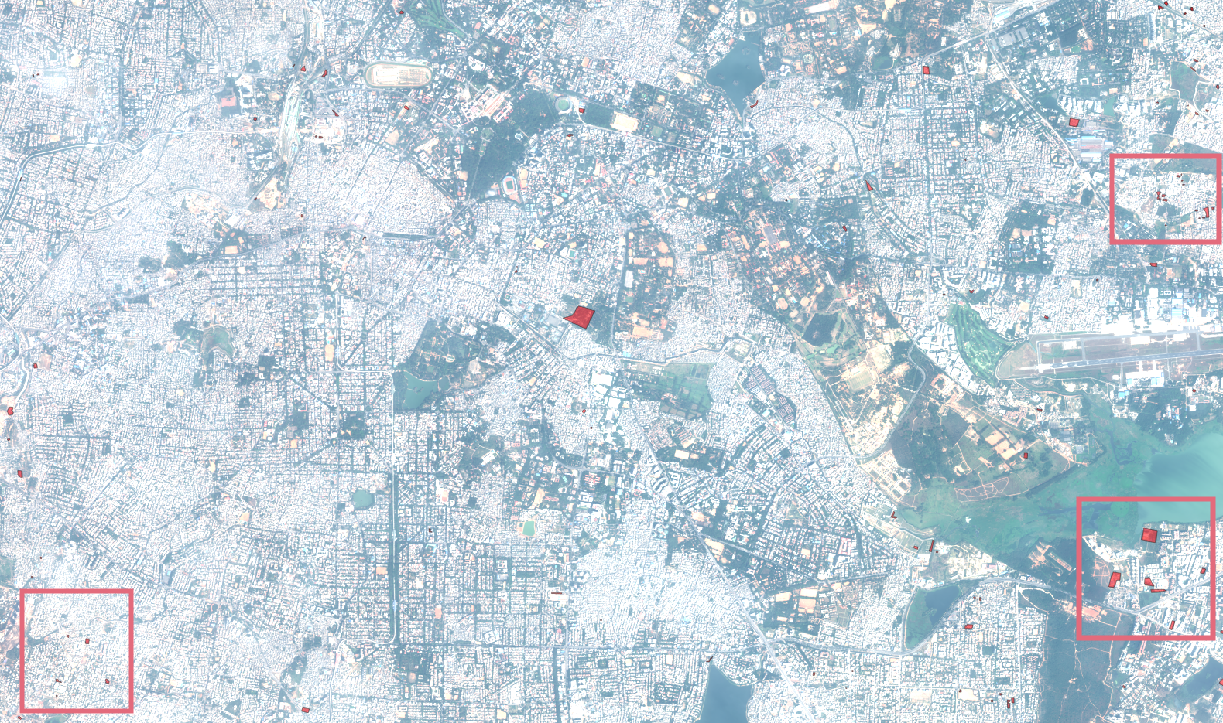
\includegraphics[width=\linewidth]{images/west-bangalore_sections}
	\caption{The entire image of West-Bangalore}
	\label{fig:ap_a_1}
\end{figure}

\section{Code}



\end{document}

Gradient-Magnitude-Based Support Regions in Structural Land Use Classification
